\chapter{Service Layer: Memory Management as a Service}
\label{chap:service}

\begin{figure}[t]
  \centering
  \subfigure[\scriptsize Intermediate data (normalized by mean usage)] {
    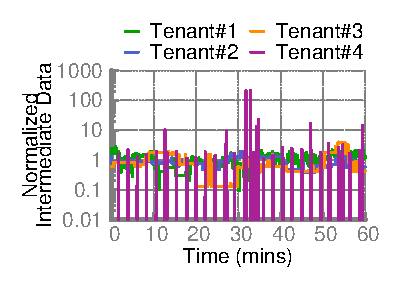
\includegraphics[width = 0.45\textwidth]{fig/jiffy/ephemeral_avg}
    \label{fig:ephemeral-avg}
  }
  \subfigure[\scriptsize Cumulative intermediate data (normalized by peak usage)] {
    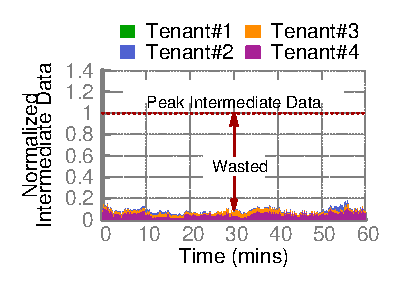
\includegraphics[width = 0.45\textwidth]{fig/jiffy/ephemeral}
    \label{fig:ephemeral-cum}
  }
  \caption[Snowflake workload anaylsis.]{\small{Analysis of production workloads from Snowflake~\cite{snowset} for four tenants over a $1$ hour window: (a) the ratio of peak to average storage usage for a job can vary by an order of magnitude during its execution; and (b) provisioning for peak usage results in average utilization $<10\%$. Across all tenants, the average utilization is $19\%$.}}\label{fig:ephemerals}%\vspace{-1.25em}
\end{figure}

Today's cloud applications rely heavily on the service layer~\cite{service1, service2, service3, service4, service5}, which sits above the OS layer and is divided into three sub-layers: Infrastructure as a Service (IaaS), Platform as a Service (PaaS), and Software as a Service (SaaS). Infrastructure as a Service (IaaS)~\cite{iaas1, iaas2} is a model where organizations outsource essential computing resources—such as storage, hardware, servers, and networking—to a service provider. The provider manages and maintains the infrastructure, while clients typically pay based on usage. This layer offers greater flexibility compared to the OS, enabling it to provide adaptable services that cater to the specific needs of various applications. However, this flexibility may require significant modifications to applications that do not utilize similar programming interfaces.

Migrating general cloud applications to disaggregated architectures presents challenges due to the substantial differences in the underlying infrastructure, such as physically decoupled resources and performance variability within interconnects. Rather than directly modifying applications to accommodate these new architectures, a more efficient approach is to provide \textbf{Memory Management as a Service} (MMaaS), which can be utilized by multiple applications. 

In this chapter, we begin by exploring the memory management service design for data analytics applications in serverless computing~\cite{starling, locus, pocket, flint, sparkonlambda, cirrus, excamera, pywren, numpywren, gg, athena, aurora, azuresqldw, cloudburst, snowset, caerus}. Recent advances in serverless analytics have shown the benefits of leveraging serverless architectures for resource- and cost-efficient data analytics. In these systems, remote, low-latency, high-throughput disaggregated memory is employed to store intermediate states for inter-task\footnote{Despite differences in their underlying programming models and semantics, existing distributed programming frameworks share a common structure (Figure~\ref{fig:example}). Specifically, a job is divided into multiple \textit{tasks}, which may be organized into several stages or structured as a directed acyclic graph (DAG). During execution, each task produces \textit{intermediate} data, which is partitioned upon task completion. This partitioned data is then exchanged with tasks in subsequent stages, enabling efficient data processing across the distributed system.} communication and multi-stage jobs, extending the lifetime of data beyond the task that produced it. This natural separation of compute and memory makes serverless computing an ideal candidate for harnessing disaggregated memory architectures.


Serverless analytics applications\cite{starling, shuffling, pocket, cirrus} handle user requests in the form of jobs, each defining its memory needs upon creation. The dilemma of balancing performance with resource efficiency for job-level memory allocation has been extensively studied ~\cite{elasticquery, qoop}. If a job is based on average demand, performance may decline during peak demand periods due to inadequate memory, causing data spillage to slower secondary storage, such as SSDs. Conversely, allocating memory for peak demands leads to underutilization of resources when the actual demand is below peak. Evaluations on Snowflake's workload, as shown in ~\cite{elasticquery}, indicate a significant fluctuation in the ratio of peak to average demands, sometimes varying by two orders of magnitude within minutes.

Designing a memory management service for such systems is a non-trivial task. We begin by outlining the essential requirements for memory management in disaggregated environments, focusing on the unique challenges posed by disaggregation:

\paragraphb{Elasticity}  Memory usage in modern computing is highly variable, with applications facing fluctuating demands~\cite{jiffy}. Elasticity enables dynamic memory allocation based on current needs, optimizing resource utilization. Applications like data analytics consist of jobs with multiple tasks that communicate via intermediate memory. Traditional solutions allocate memory at the job level, where jobs specify their requirements before execution, and the system reserves that amount for the job's duration~\cite{pocket}. This approach creates a tradeoff: allocating for average demand risks performance degradation due to swapping data to slower storage (e.g., S3), as shown in Figure~\ref{fig:ephemeral-avg}, while allocating for peak demand leads to resource waste (Figure~\ref{fig:ephemeral-cum}). Recent studies report that intermediate data sizes can vary by orders of magnitude during a job's lifetime~\cite{snowset}. For example, Figure~\ref{fig:ephemerals} shows that in a Snowflake dataset with over 2000 tenants, peak-to-average memory demand can vary by two orders of magnitude within minutes, resulting in performance degradation and resource inefficiency in job-level allocations.

\paragraphb{Isolation} The second requirement is the isolation between different compute tasks. Since multiple computing threads can be using the same disaggregated memory pool, it's essential to multiplex between applications to improve resource efficiency but at the same time keep the memory of different threads isolated from each other, which means that the memory usage of a particular application should not affect other existing applications. The number of tasks reading and writing to the shared disaggregated memory can change rapidly in serverless analytics which makes the problem even more severe.

\paragraphb{Lifetime management}
Decoupling compute tasks from their intermediate storage means that the tasks can fail independent of the intermediate data, therefore we need mechanisms for explicity lifetime management of intermediate data.

\paragraphb{Data repartitioning}
Decoupling tasks from their intermediate data also means that data partitioning upon elastic scaling of memory capacity becomes challenging, especially for certain data types used in serverless analytics (e.g. key-value store). If it's the application's responsibility to perform such repartitioning, it will involve large network transfers betweem compute tasks and the far memory system and massive read/write operations every time the capacity is scaled. What's more, the application need to implement different partitioning strategies for different kind of data structures used. Therefore, new mechansims to efficiently enable data partitioning within the far memory system is essential.


We present Jiffy, an elastic disaggregated-memory system for stateful serverless analytics. Jiffy allocates memory resources at the granularity of small fixed-size memory blocks - multiple memory blocks store intermediate data for individual tasks within a job. Jiffy design is motivated by virtual memory design in operating systems that also does memory allocation to individual process at the granularity of fixed-size memory blocks(pages). Jiffy adapts this design to stateful serverless analytics. Performing resource allocation at the granularity of small memory blocks allows Jiffy to elastically scale memory resources allocated to individual jobs without a priori knowledge of intermediate data sizes and to meet the instantaneous job demands at seconds timescales. As a result, Jiffy can efficiently multiplex the available faster memory capacity across concurrently running jobs, thus minimizing the overheads of reads and writes to significantly slower secondary storage (e.g., S3 or disaggregated storage)


\begin{figure}
  \centering
  \begin{tikzpicture}[font=\scriptsize, yscale=0.8, task/.style={draw, circle, align=center, inner sep=2pt}]
    \node[task] (t1) {\texttt{T1}};
    \node[task, above=0.25em of t1] (t2) {\texttt{T2}};
    \node[task, above=0.25em of t2] (t3) {\texttt{T3}};
    \node[task, above=0.25em of t3] (t4) {\texttt{T4}};
    \node[task, right=1.5em of t1, yshift=2em] (t5) {\texttt{T5}};
    \node[task, right=1.5em of t3, yshift=1em] (t6) {\texttt{T6}};
    \node[task, right=4.75em of t3, yshift=-0.5em] (t8) {\texttt{T7}};
    \node[task, right=8em of t2, yshift=-1em] (t10) {\texttt{T8}};
    \node[task, right=8em of t4, yshift=-1em] (t12) {\texttt{T9}};
    
    
    \draw[-stealth] (t1.east) -- (t5.west);
    \draw[-stealth] (t2.east) -- (t5.west);
    \draw[-stealth] (t3.east) -- (t8.west);
    \draw[-stealth] (t4.east) -- (t6.west);
    \draw[-stealth] (t5.east) -- (t8.west);
    \draw[-stealth] (t6.east) -- (t8.west);
    \draw[-stealth] (t8.east) -- (t10.west);
    \draw[-stealth] (t8.east) -- (t12.west);
    
    \node[draw, fill=gray!10, left=2.25em of $(t3)!0.5!(t2)$] {\rotatebox{90}{Persistent Storage}\rotatebox{90}{\quad\quad(\eg, S3)}};
    \node[draw, fill=gray!10, right=11.75em of $(t3)!0.5!(t2)$] {\rotatebox{90}{Persistent Storage}\rotatebox{90}{\quad\quad(\eg, S3)}};
    
    \draw[-stealth] ($(t1.west)+(-1.6em, 0)$) -- (t1.west);
    \draw[-stealth] ($(t2.west)+(-1.6em, 0)$) -- (t2.west);
    \draw[-stealth] ($(t3.west)+(-1.6em, 0)$) -- (t3.west);
    \draw[-stealth] ($(t4.west)+(-1.6em, 0)$) -- (t4.west);
    \draw[-stealth] (t10.east) -- ($(t10.east)+(1.5em, 0)$);
    \draw[-stealth] (t12.east) -- ($(t12.east)+(1.5em, 0)$);
    
    \node[task, above=0.5em of t4, xshift=-1em] (tl) {};
    \node[right=0em of tl] (t) {Task};
    \node[right=2em of t] {Intermediate Data Exchange};
    \draw[-stealth] ($(t)+(2em, 0em)$) -- ($(t)+(3em, 0em)$);
    
  \end{tikzpicture}
  \caption[Execution DAG example for a typical analytics job.]{\small\textbf{Execution DAG example for a typical analytics job.} Intermediate data exchange across tasks occurs via \jiffy.}
  \label{fig:example}
  \label{fig:query-example}
\end{figure}

\section{\jiffy Design}
\label{sec:jiffydesign}

This section explains how \jiffy uses hierarchical addressing, intermediate data lifetime management, and flexible data repartitioning to meet these requirements. We illustrate this with Figure~\ref{fig:query-example}, which depicts the execution plan of a typical analytics job. The plan is represented as a directed acyclic graph (DAG), where nodes are computation tasks (implemented as serverless functions\footnote{Functions refer to basic computation units in serverless architectures, such as Amazon Lambdas~\cite{alambda}, Google Functions~\cite{googlefunctions}, and Azure Functions~\cite{azureFunctions}}), and edges represent intermediate data exchanged via \jiffy.


\begin{figure}[t]
  \centering
  \begin{tikzpicture}[font=\scriptsize, yscale=0.75, task/.style={draw, circle, align=center, inner sep=2pt}, block/.style={draw, align=center, fill=gray!20, inner sep=2pt}]
    \node[task] (t1) {\texttt{T1}};
    \node[task, right=1.5em of t1] (t2) {\texttt{T2}};
    \node[task, right=1.5em of t2] (t3) {\texttt{T3}};
    \node[task, right=1.5em of t3] (t4) {\texttt{T4}};
    \node[task, below=0.5em of t1, xshift=2em] (t5) {\texttt{T5}};
    \node[task, below=0.5em of t4] (t6) {\texttt{T6}};
    \node[task, below=2.75em of t3, xshift=-0.5em] (t8) {\texttt{T7}};
    \node[task, below=5em of t2] (t10) {\texttt{T8}};
    \node[task, below=5em of t4] (t12) {\texttt{T9}};
    
    \node[block, above=0.25em of t3, xshift=-1em] (t3b1) {\texttt{B3\_1}};
    \node[block, above=0.25em of t3, xshift=1em] (t3b2) {\texttt{B3\_2}};
    \node[block, left=0.5em of t5] (t5b1) {\texttt{B5\_1}};
    \node[block, right=0.5em of t6, yshift=0.5em] (t6b1) {\texttt{B6\_1}};
    \node[block, right=0.5em of t6, yshift=-0.5em] (t6b2) {\texttt{B6\_2}};
    \node[block, right=0.5em of t8] (t8b1) {\texttt{B7\_1}};

    \draw[-stealth] (t1.south) -- (t5.north);
    \draw[-stealth] (t2.south) -- (t5.north);
    \draw[-stealth] (t3.south) -- (t8.north);
    \draw[-stealth] (t4.south) -- (t6.north);
    \draw[-stealth] (t5.south) -- (t8.north);
    \draw[-stealth] (t6.south) -- (t8.north);
    \draw[-stealth] (t8.south) -- (t10.north);
    \draw[-stealth] (t8.south) -- (t12.north);
    
    \draw[-stealth] (t3.north) -- (t3b1.south);
    \draw[-stealth] (t3.north) -- (t3b2.south);
    \draw[-stealth] (t5.west) -- (t5b1.east);
    \draw[-stealth] (t6.east) -- (t6b1.west);
    \draw[-stealth] (t6.east) -- (t6b2.west);
    \draw[-stealth] (t8.east) -- (t8b1.west);
    
    \draw[thick, dashed, opacity=0] ($(t5.south west)+(-0.3em, -0.3em)$) rectangle node[midway, right] (t5a) {} ($(t5.north east)+(2.05em, 0.3em)$);
    \draw[thick, dashed, opacity=0, fill=red, fill opacity=0.2] ($(t6.south west)+(-0.3em, -0.75em)$) rectangle node[midway, right] (t6a) {} ($(t6.north east)+(2.75em, 0.75em)$);
    \draw[thick, dashed, opacity=0, fill=red, fill opacity=0.2] ($(t8.south west)+(-0.3em, -0.3em)$) rectangle node[midway, right] (t8a) {} ($(t8.north east)+(2.75em, 0.3em)$);
    
    \node[right=4em of t8a, text width=3em, align=center] (ri) {Task-level Isolation};
    \draw[-stealth, dashed] (ri.west) -- ($(t8a.east)+(1em,0em)$);
    \draw[-stealth, dashed] (ri.north) -- ($(t6a.east)+(1em,0em)$);
    
  \end{tikzpicture}
  \caption[Hierarchical addressing]{\textbf{Hierarchical addressing} for the job in Figure~\ref{fig:query-example}. \jiffy provides task-level resource isolation for ephemeral storage under each task address-prefix (\S\ref{ssec:hva}). Note that block addresses are only assigned to address-prefixes with currently allocated blocks; for tasks \texttt{T1}, \texttt{T2} and \texttt{T4}, blocks are directly read from persistent storage and not stored in \jiffy.}
  \label{fig:hina}
\end{figure}

\subsection{Hierarchical Addressing}
\label{ssec:hva}
Analytics jobs are often structured as multiple stages or a directed acyclic graph (DAG). In serverless analytics, where compute elasticity is key, each job can run tens to thousands of tasks~\cite{starling, locus, pocket, flint, sparkonlambda, cirrus, excamera, pywren, numpywren, gg, athena, aurora, azuresqldw, cloudburst, snowset}. Fine-grained resource allocation requires efficient mapping between tasks and their storage blocks, especially with rapidly changing task concurrency. High concurrency demands task-level isolation, ensuring that task arrival or departure doesn't affect others, avoiding performance degradation.

\jiffy adopts a hierarchical addressing mechanism, inspired by the Internet's IP addressing, to maintain task-to-storage mappings and ensure task-level isolation. \jiffy organizes intermediate data in a virtual address hierarchy based on task dependencies in the DAG. Internal nodes represent tasks, and leaf nodes represent \jiffy blocks storing data. Block addresses are defined by the hierarchy path, with task-generated prefixes. Dependencies between tasks are captured by edges between nodes. \jiffy builds this hierarchy from execution plans (e.g., AWS Step Functions, Azure Durable Functions) or dynamically deduces it via the \jiffy API, supporting dynamic query plans without predefined DAGs.

\paragraphb{Example} Figure~\ref{fig:hina} illustrates the \lh for the job in Figure~\ref{fig:example}. Internal nodes \texttt{T1}-\texttt{T9} represent tasks in the DAG, while leaf nodes \texttt{B3\_1}, \texttt{B3\_2}, etc., represent data blocks allocated by \jiffy for intermediate data storage. Edges like (\texttt{T1}, \texttt{T5}) and (\texttt{T2}, \texttt{T5}) indicate that \texttt{T5} depends on the intermediate data from both \texttt{T1} and \texttt{T2}. The full address of block \texttt{B6\_2} under \texttt{T6} is \texttt{T4.T6.B6\_2}, with \texttt{T4.T6} identifying all blocks under \texttt{T6}. \jiffy constructs the \lh either using the execution plan from Figure~\ref{fig:query-example} or deduces it dynamically. For instance, \sl can infer that since \texttt{T7}'s sub-tasks access data from \texttt{T3}, \texttt{T5}, and \texttt{T6}, these tasks must be its parents in the hierarchy.


By organizing intermediate data in a hierarchy, \jiffy manages resource allocation per address prefix. If one prefix spills to persistent storage (via Pocket), it doesn’t affect others. Blocks remain assigned until reclaimed or leases expire (\S\ref{ssec:mlm}), ensuring task-level isolation regardless of churn. Like virtual memory isolating processes, \jiffy uses hierarchical addressing to isolate tasks based on the job's structure.

Two design considerations arise: (1) \jiffy's fine-grained allocation is independent of fairness policies, which can be layered on top, and (2) address translation from virtual to physical storage happens at a centralized metadata server (like Pocket~\cite{pocket}), scaling to arbitrary DAG sizes. Despite added complexity, \jiffy scales to ${\sim}45$K requests/sec/core, sufficient for most deployments.

\paragraphb{Block sizing} Jiffy balances metadata storage and memory use with block sizes, like $128$MB in HDFS~\cite{hdfs}. Larger blocks reduce metadata but risk fragmentation, while smaller blocks improve utilization at a metadata cost. Jiffy mitigates this via fine-grained access and data repartitioning.

\paragraphb{Isolation granularity} Task-level isolation, where nodes in the hierarchy map to tasks, is default, but finer or coarser isolation (e.g., table-level or stage-level) can be configured via the \jiffy API.


\subsection{Data Lifetime Management}
\label{ssec:mlm}

\begin{figure}[t]
  \centering
  \begin{tikzpicture}[font=\scriptsize, yscale=0.75, task/.style={draw, circle, align=center, inner sep=2pt}, block/.style={draw, align=center, fill=gray!20, inner sep=2pt}]
    \node[task] (t1) {\texttt{T1}};
    \node[task, right=1.5em of t1] (t2) {\texttt{T2}};
    \node[task, fill=BurntOrange!30, right=1.5em of t2] (t3) {\texttt{T3}};
    \node[task, right=1.5em of t3] (t4) {\texttt{T4}};
    \node[task, fill=BurntOrange!30, below=0.5em of t1, xshift=2em] (t5) {\texttt{T5}};
    \node[task, fill=BurntOrange!30, below=0.5em of t4] (t6) {\texttt{T6}};
    \node[task, fill=blue!30, below=2.75em of t3, xshift=-0.5em] (t8) {\texttt{T7}};
    \node[task, fill=BurntOrange!30, below=5em of t2] (t10) {\texttt{T8}};
    \node[task, fill=BurntOrange!30, below=5em of t4] (t12) {\texttt{T9}};
    
    \node[block, fill=BurntOrange!50, above=0.25em of t3, xshift=-1em] (t3b1) {\texttt{B3\_1}};
    \node[block, fill=BurntOrange!50, above=0.25em of t3, xshift=1em] (t3b2) {\texttt{B3\_2}};
    \node[block, fill=BurntOrange!50, left=0.5em of t5] (t5b1) {\texttt{B5\_1}};
    \node[block, fill=BurntOrange!50, right=0.5em of t6, yshift=0.5em] (t6b1) {\texttt{B6\_1}};
    \node[block, fill=BurntOrange!50, right=0.5em of t6, yshift=-0.5em] (t6b2) {\texttt{B6\_2}};
    \node[block, fill=BurntOrange!50, right=0.5em of t8] (t8b1) {\texttt{B7\_1}};

    \draw[-stealth] (t1.south) -- (t5.north);
    \draw[-stealth] (t2.south) -- (t5.north);
    \draw[-stealth] (t3.south) -- (t8.north);
    \draw[-stealth] (t4.south) -- (t6.north);
    \draw[-stealth] (t5.south) -- (t8.north);
    \draw[-stealth] (t6.south) -- (t8.north);
    \draw[-stealth] (t8.south) -- (t10.north);
    \draw[-stealth] (t8.south) -- (t12.north);
    
    \draw[-stealth] (t3.north) -- (t3b1.south);
    \draw[-stealth] (t3.north) -- (t3b2.south);
    \draw[-stealth] (t5.west) -- (t5b1.east);
    \draw[-stealth] (t6.east) -- (t6b1.west);
    \draw[-stealth] (t6.east) -- (t6b2.west);
    \draw[-stealth] (t8.east) -- (t8b1.west);
    
    \draw[thick, dashed, opacity=0] ($(t8.south west)+(-0.3em, -0.3em)$) rectangle node[midway, right] (t8a) {} ($(t8.north east)+(2.05em, 0.3em)$);
%    
    \node[circle, fill=blue!30, right=6em of t8a, yshift=2em] (lr) {};
    \node[right=0em of lr, text width=4em] {Requested lease renewal};
    \node[circle, fill=BurntOrange!30, below=0.75em of lr] (ar) {};
    \node[right=0em of ar, text width=4em] {Automatic lease renewal};
    
  \end{tikzpicture}
  \caption[Lease Renewal via Address Hierarchy]{\textbf{Lease Renewal via Address Hierarchy.} Hierarchical addressing simplifies lease renewal in \jiffy (\S\ref{ssec:mlm}), since lease renewal for an address-prefix automatically implies renewals for all parent and descendent address-prefixes in the hierarchy.}\label{fig:mlm}
\end{figure}

Existing ephemeral storage systems manage data at the job level, reclaiming storage when the job deregisters. In serverless analytics, decoupled task execution and storage can lead to orphaned data. \jiffy addresses this by integrating lease management~\cite{gray1989leases, chubby, dhcplease} with hierarchical addressing for task-level data management. Each address prefix has a lease, and data is retained as long as the lease is renewed. Serverless platforms can trigger lease renewals during task monitoring.

Using the DAG hierarchy, \jiffy renews leases for dependent and ancestor tasks automatically, reducing overhead while preventing orphaned data. This strikes a balance between age-based eviction and explicit resource management, ensuring efficient reassignment of resources upon task or job failure.

\paragraphb{Example} In Figure~\ref{fig:query-example}, task \texttt{T7}'s job periodically renews the lease for the prefix \texttt{T4.T6.T7}\footnote{Task \texttt{T7} has four address prefixes; the job can renew any.}. Renewing \texttt{T7}'s lease also renews those for parent tasks (\texttt{T3}, \texttt{T5}, \texttt{T6}) and descendants (\texttt{T8}, \texttt{T9}), as shown in Figure~\ref{fig:mlm}. This ensures that both parent and descendant tasks' data remain accessible.

\paragraphb{Lease duration} Lease duration trades off control plane bandwidth with system utilization. Longer leases reduce network traffic but may delay resource reclamation. Configuring lease durations, as studied in prior work~\cite{chubby, gray1989leases}, allows \jiffy to meet specific deployment goals.






\subsection{Flexible Data Repartitioning}
\label{ssec:fdr}

Decoupling compute tasks from their intermediate data in serverless analytics introduces challenges in achieving fine-grained elasticity for ephemeral storage. Specifically, when storage is allocated or deallocated for a task, the intermediate data must be efficiently repartitioned across available blocks. However, due to the decoupling of compute from storage and the large number of concurrent tasks, this repartitioning should not be managed by the application itself. For instance, many serverless analytics systems~\cite{locus, pocket} rely on key-value stores for intermediate data. If compute tasks were responsible for repartitioning during memory scaling, they would need to read key-value pairs over the network, compute new partitions based on updated memory, and write the data back to the store—resulting in significant network latency and bandwidth overhead.

\jiffy supports various data structures commonly used in data analytics frameworks, including files~\cite{sparkonlambda, athena, aurora, azuresqldw, snowset}, key-value pairs~\cite{pywren, locus, starling, gg, cirrus, cloudburst, pocket}, and queues~\cite{flint, excamera}. Analytics jobs using these structures can delegate intermediate data repartitioning to \jiffy during resource allocation or deallocation. Each block in a \jiffy data structure tracks its own memory usage. When usage exceeds a predefined threshold, \jiffy allocates a new block to the corresponding address-prefix\footnote{Similar to existing systems~\cite{elasticache, redis, ramcloud, pocket}, \sl can scale cluster capacity by adding or removing servers based on free blocks. Here, we focus on fine-grained elasticity.}. The overloaded block triggers a data-specific repartitioning process, moving some of its data to the newly allocated block. Conversely, when block usage drops below a low threshold, \jiffy merges it with another low-usage block before deallocating the unused block. By allowing the block itself, rather than the compute task, to handle repartitioning, \jiffy minimizes network and compute overhead for the task. Repartitioning is done asynchronously, allowing data access to continue with minimal impact on performance.

Jiffy’s supported data structures enable the serverless execution of powerful distributed frameworks like MapReduce~\cite{mapreduce,spark}, Dryad~\cite{dryad}, StreamScope~\cite{streamscope}, and Piccolo~\cite{piccolo}. Since files, queues, and key-value stores in analytics frameworks require relatively simple repartitioning (unlike complex structures such as B-trees), serverless applications can leverage \jiffy’s flexible repartitioning mechanism without requiring any modifications.


\paragraphb{Thresholds for Elastic Scaling} In \jiffy, the high and low thresholds play a crucial role in balancing network bandwidth usage, task performance, and overall system utilization. Setting thresholds too high or too low can impact elastic scaling behavior—if scaling is triggered too infrequently, it may reduce network traffic, but it can also result in inefficient block utilization, such as numerous underutilized blocks. The optimal values for these thresholds depend heavily on the specific workload characteristics, as highlighted in previous studies~\cite{mongo-shard, ceph-shard}. To accommodate diverse workloads, \jiffy makes these thresholds fully configurable, allowing users to adjust them to suit their performance and efficiency needs.


\section{\jiffy Implementation}
\label{sec:jiffyimplementation}

\jiffy builds on Pocket~\cite{pocket}, inheriting its scalable and fault-tolerant metadata plane, multi-tiered data storage, system-wide capacity scaling, and analytics execution model. However, \jiffy introduces hierarchical addressing, lease management, and efficient data repartitioning to address the unique challenges of serverless environments. Below, we describe the \jiffy interface and implementation, highlighting these key features.

\subsection{\jiffy Interface}
\label{ssec:jiffyapi}

\begin{table}[t]
    \centering
    \footnotesize
    \begin{tabular}{c|l}
        \hline
        \textbf{API Group} & \textbf{Function Signature} \\
        \hline
        \multicolumn{1}{c|}{} & connect(honeycombAddress) \\
        \hline
        \multirow{4}{*}{Address Hierarchy} 
            & createAddrPrefix(addr, parent, optionalArgs) \\
            & createHierarchy(dag, optionalArgs) \\
            & flushAddrPrefix(addr, externalPath) \\
            & loadAddrPrefix(addr, externalPath) \\
        \hline
        \multirow{2}{*}{Lease Operations} 
            & leaseDuration = getLeaseDuration(addr) \\
            & renewLease(addr) \\
        \hline
        \multirow{3}{*}{Data Structure}
            & ds = initDataStructure(addr, type) \\
            & listener = ds.subscribe(op) \\
            & notif = listener.get(timeout) \\
        \hline
    \end{tabular}
    \caption[\jiffy User-facing API]{\textbf{\jiffy User-facing API}: Functions for connecting, managing address hierarchies, handling leases, and interacting with data structures.}
    \label{table:api}
\end{table}



We describe the \jiffy interface in terms of its user-facing API (Table~\ref{table:api}) and internal API (Figure~\ref{fig:blockapi}).

\paragraphb{User-facing API} The user-facing interface (Table~\ref{table:api}) is centered around two core abstractions: \textit{hierarchical addresses} and \textit{data structures}. Jobs can create a new address-prefix using \texttt{createAddrPrefix}, specifying the parent prefix along with optional parameters such as initial capacity. The \texttt{createHierarchy} function generates a complete hierarchy from an execution plan (DAG), while \texttt{flush} and \texttt{load} facilitate persisting and retrieving address-prefix data from external storage (e.g., S3). Three built-in data structures can be initialized for an address-prefix via \texttt{initDataStructure}, and new structures can be defined using the internal API.

Similar to existing systems~\cite{redis, sns}, \jiffy’s data structures provide a notification interface, allowing tasks that consume intermediate data to be informed when new data is available. For example, a task can \texttt{subscribe} to write operations on its parent task’s data structure and receive a \texttt{listener} handle. When data is written, \jiffy asynchronously notifies the \texttt{listener}, which the task can access via \texttt{listener.get()}.


\begin{figure}[h]
  \centering
  \begin{tabular}{c}
  {\begin{lstlisting}[frame=single, gobble=4, linewidth=20em]
    block = ds.getBlock(op, args) // Get block
    block.writeOp(args) // Perform write
    data = block.readOp(args) // Perform read
    block.deleteOp(args) // Perform delete
  \end{lstlisting}}
  \end{tabular}
  \caption[\jiffy Internal API]{\textbf{\jiffy Internal API.} The block interface is used internally in \jiffy to implement the data structure APIs.}  
  \label{fig:blockapi}
\end{figure}

\paragraphb{Internal API} The data layout within \jiffy blocks is tailored to the specific data structure that owns it. Therefore, \jiffy blocks expose a set of data structure-specific \textit{operators} (Figure~\ref{fig:blockapi}) that define how requests are \textit{routed} across blocks and how data is \textit{accessed} or \textit{modified}. These operators are used internally by \jiffy for its built-in data structures (\S\ref{ssec:jiffymodels}) and are not directly exposed to jobs.

The \texttt{getBlock} operator determines the target block for an operation based on the operation type and its arguments (e.g., key hashes for a KV-store), returning a handle to the appropriate block. Each \jiffy block provides \texttt{writeOp}, \texttt{readOp}, and \texttt{deleteOp} operators, which implement data structure-specific access logic (e.g., \texttt{get}, \texttt{put}, and \texttt{delete} in a KV-store). Jiffy executes these operators \textit{atomically} using sequence numbers but does not support atomic transactions across multiple operators.



\begin{table*}[t]
  \centering
  \small
  \caption[\jiffy Data Structure Implementations]{\textbf{\jiffy Data Structure Implementations}. See \S\ref{ssec:jiffymodels} for details.}
  \label{table:ds}
  \begin{tabular}{c|l|c|c|c|l|c}
    \hline
    \multicolumn{2}{c|}{\textbf{Data Structure}} & \textbf{writeOp} & \textbf{readOp} & \textbf{deleteOp} & \textbf{getBlock} & \textbf{repartition} \\
    \hline
    \hline
    \multirow{3}{*}{\rotatebox[origin=c]{90}{\footnotesize Built-in}} 
      & File (\S\ref{sssec:bsp}) & \texttt{write} & \texttt{read} & \texttt{-} & File offsets. & \xmark \\\cline{2-7}
      & FIFO Queue (\S\ref{sssec:dflow}) & \texttt{enqueue} & \multicolumn{2}{c|}{\texttt{dequeue}} & Tail/head. & \xmark \\\cline{2-7}
      & KV-Store (\S\ref{sssec:piccolo}) & \texttt{put} & \texttt{get} & \texttt{delete} & Key hash. & \checkmark \\
    \hline
    \multicolumn{7}{c}{\textit{Custom data structures}} \\
    \hline
  \end{tabular}
\end{table*}


\begin{figure}[h]
  \centering
  \begin{tikzpicture}[font=\scriptsize, yscale=0.9, level distance=1.7em, level 1/.style={sibling distance=3em}, level 2/.style={sibling distance=3em}, level 3/.style={sibling distance=3em}]
  	\node (root) [draw, text width=5em, align=center] {Job to address\\prefix mapping}
  	   child { node[fill=gray!10] (app1) {\aa}
        child { node[fill=gray!10] (g1) {\texttt{T1}} 
          child { node[fill=gray!10] (task1) {\texttt{T3}} }
          child { node {...} }
        }
        child { node[fill=gray!10] (g2) {\texttt{T2}} 
          child { node (r) {...} }
        }
      }
      child {
        node[fill=gray!10] (app2) {\ab}
        child { node {...} }
      };
    \draw[black, thick, color=gray] ($(app1.north west)+(-3.25em,2.25em)$) rectangle node[midway, right] (tree-border) {} ($(r.south east)+(2.5em,-0.5em)$);
  	\node[draw, dotted, fill=gray!10, text width=3.5em, align=center, left=0.25em of g1.north west, yshift=1.75em] (internal) {children, permissions, timestamp, blocks, ...};
  	\draw[dotted] ($(g1.north west)+(1em, 0em)$) -- (internal.north east);
  	\draw[dotted] (g1.north west) -- (internal.south east);
  	

    \node[draw, below=0.75em of r.south east, xshift=-2.9em] (head) {};
    \node[draw, right=0.5em of head] (mid1) {};
    \node[draw, right=0.5em of mid1] (mid2) {};
    \node[draw, right=0.5em of mid2] (mid3) {};
    \node[draw, right=0.5em of mid3] (tail) {};

    \draw[-latex] (head.east) -- (mid1.west);
    \draw[-latex] (mid1.east) -- (mid2.west);
    \draw[-latex] (mid2.east) -- (mid3.west);
    \draw[-latex] (mid3.east) -- (tail.west);

    \node[left=-0.25em of head] (flist) {Free List};

    \draw[black, thick, color=gray] ($(flist.north west)+(0.15em, 0em)$) rectangle ($(tail.south east)+(0.2em, -0.25em)$);
  	
  	\node[draw, fill=green!30, text width=5.5em, align=center] (fs-api) at ([xshift=8em, yshift=2.55em]tree-border){$\strut$Metadata Manager};
  	
  	\node[draw, fill=BurntOrange!20, minimum height=4em, text width=5.5em, align=center, below=0.1em of fs-api] (lm) {};
  	\node[text width=5.5em, align=center, below=-0.1em of lm.north] (lm-title) {Lease Manager};
  	\node[draw, fill=BurntOrange!50, text width=5.4em, align=center, below=-0.1em of lm-title] (lm-renewal) {Renewal Service};
  	\node[draw, fill=BurntOrange!50, text width=5.4em, align=center, below=0.1em of lm-renewal] (lm-expiry) {Expiry Worker};
  	
  	\node[draw, fill=blue!30, minimum height=1em, text width=5.5em, align=center, below=0.1em of lm] (sm) {$\strut$Block Allocator};
  	
  	\draw[black, thick, color=gray] ($(app1.north west)+(-6.25em,2.4em)$) rectangle node[midway, right] (dir-border) {} ($(sm.south east)+(0.4em,-0.75em)$);
  	
  	\node[draw, dashed, text width=2.5em, align=center, right=1em of fs-api] (client) {Client};
  	\node[draw, dashed, text width=2.5em, align=center, right=1em of sm] (ss) {Data Plane};
  	
  	\draw[stealth-stealth, thick] (fs-api.east) -- (client.west);
  	\draw[stealth-stealth, thick] (lm-renewal.east) -- (client.west);
  	\draw[stealth-stealth, thick] (sm.east) -- (client.west);
  	\draw[stealth-stealth, thick] (fs-api.east) -- (ss.west);
  	\draw[stealth-stealth, thick] (lm-expiry.east) -- (ss.west);
  	\draw[stealth-stealth, thick] (sm.east) -- (ss.west);
  	
  	\draw[stealth-stealth, thick] (fs-api.west) -- ($(fs-api.west)+(-1em, 0em)$);
  	\draw[stealth-stealth, thick] (lm.west) -- ($(lm.west)+(-1em, 0em)$);
  	\draw[stealth-stealth, thick] ($(sm.west)+(0em,0.5em)$) -- ($(sm.west)+(-1em, 0.5em)$);
    \draw[stealth-stealth, thick] ($(sm.west)+(0em,-0.5em)$) -- ($(sm.west)+(-1em, -0.5em)$);
	
  \end{tikzpicture}
  \caption[\jiffy controller]{\small\textbf{\jiffy controller.} See \S\ref{sec:cp} for details.}
  \label{fig:ds-arch}
\end{figure}
%
\subsection{System Implementation}
\label{sec:cp}
\label{sec:dp}

Since \jiffy design builds on Pocket, its high-level design components are also similar, except for one difference: \jiffy combines the control and metadata planes into a unified control plane. We found this design choice allowed us to significantly simplify interactions between the control and metadata components, without affecting their performance. While this does couple their fault-domains, standard fault-tolerance mechanisms (\eg, the one outlined in~\cite{pocket}) are still applicable to the unified control plane. 


\paragraphb{Control plane} The \jiffy controller (Figure~\ref{fig:ds-arch}) maintains two pieces of system-wide state. First, it stores a \textit{free block list}, which lists the set of blocks that have not been allocated to any job yet, along with their corresponding physical server addresses. Second, it stores an {\lh} per-job, where each node in the hierarchy stores variety of metadata for its address-prefix, including access permissions (for enforcing access control), timestamps (for lease renewal), a block-map (to locate the blocks associated with the address-prefix in the data plane), along with metadata to identify the data structure associated with the address-prefix and how data is partitioned across its blocks. The mapping between jobIDs (which uniquely identify jobs) and their address hierarchies is stored in a hash-table at the controller.

\begin{figure}
  \centering
  \begin{tikzpicture}[font=\scriptsize, yscale=0.7]
    \node[draw, thick, minimum width=4.5em, minimum height=3.25em] (server1) {};
    \node[draw, thick, minimum width=4em, below=0.25em of server1.north] (block11) {};
    \node[fill=gray!40, minimum width=3.675em, inner sep=3pt] at ([xshift=-0.125em]block11) {};
    \node[draw, thick, minimum width=4em, below=0.25em of block11] (block12) {};
    \node[fill=gray!40, minimum width=1.925em, inner sep=3pt] at ([xshift=-1em]block12) {};
    \node[draw, thick, minimum width=4em, below=0.25em of block12] (block13) {};
    \node[fill=gray!40, minimum width=2.925em, inner sep=3pt] at ([xshift=-.5em]block13) {};
    
    \node[text width=4em, align=center, below=0em of server1] {\textbf{Server\#1}};
    
    \node[left=1em of server1] (block) {\textbf{Blocks}};
    \draw[-stealth, thick] (block) -- (block11.west);
    \draw[-stealth, thick] (block) -- (block12.west);
    \draw[-stealth, thick] (block) -- (block13.west);
    
    \draw[thick, dashed] ($(block11.north)+(1.5em, 0.5em)$) -- ($(block13.south)+(1.5em, -1em)$)node [anchor=north] (ht-line) {};
    
    \node[text width=4.5em, align=center, right=0.75em of block13, yshift=-0.5em] (ht) {High threshold};
    
    \draw[-stealth, thick] ($(ht.west)+(0.35em, 0em)$) to [out=225, in=0] (ht-line.north);
    
    \node[draw, thick, minimum width=4.5em, minimum height=3.25em, right=10em of server1] (server2) {};
    \node[draw, thick, minimum width=4em, below=0.25em of server2.north] (block21) {};
    \node[draw, thick, minimum width=4em, below=0.25em of block21] (block22) {};
    \node[fill=gray!40, minimum width=1.925em, inner sep=3pt] at ([xshift=-1em]block22) {};
    \node[draw, thick, minimum width=4em, below=0.25em of block22] (block23) {};
    \node[fill=gray!40, minimum width=1.925em, inner sep=3pt] at ([xshift=-1em]block23) {};
    
    \node[text width=4em, align=center, below=0em of server2] {\textbf{Server\#2}};
    
    \node[draw, thick, dashed, text width=6em, minimum height=1em, align=center, above=3em of $(server1)!0.5!(server2)$] (cp) {\textbf{Control Plane}};
    
    \draw[thick, color=red, -stealth] (block11.north) to [out=90, in=180] node [left, text width=4em, align=center] {\textcolor{red}{\textcircled{1}} Overload signal} (cp.west);
    
    \draw[thick, color=blue, stealth-stealth] (cp.east) to [out=0, in=90] node [right, text width=4em, xshift=0.25em, align=center] {\textcolor{blue}{\textcircled{2}} Allocate \texttt{newBlock}} (block21.north);
    
    \draw[thick, color=violet, -stealth] (cp.south) -- node [right, text width=7em, align=center, yshift=-0.25em] {\textcolor{violet}{\textcircled{3}} \texttt{newBlock} address} ($(block11.east)+(0em, 0.5em)$);
    
    \draw[thick, color=BurntOrange, -stealth] (block11.east) -- node[midway, below, align=center] {\textcolor{BurntOrange}{\textcircled{4}} Repartition data to \texttt{newBlock}} (block21.west);
  \end{tikzpicture}
  \caption[Data repartitioning on scaling up capacity]{\small\textbf{Data repartitioning on scaling up capacity.} Scaling down capacity employs a similar approach (\S\ref{sec:dp}).}\label{fig:autoscaling}
\end{figure}
%
While the block allocator and metadata manager are similar to their counterparts in Pocket, the lease manager implements lifetime management in \jiffy. It comprises a lease renewal service that listens for renewal requests from jobs and updates the lease renewal timestamp of relevant nodes in its \lh, and a lease expiry worker that periodically traverses all address hierarchies, marking nodes with timestamps older than the associated lease period as expired. Finally, \jiffy adopts mechanisms from Pocket to facilitate control plane scaling and fault tolerance; we refer the reader to~\cite{pocket} for details.

\paragraphb{Data plane} \jiffy data plane is responsible for two main tasks: providing jobs with efficient, data-structure specific atomic access to data, and repartitioning data across blocks allocated by the control plane during resource scaling. It partitions the resources in a pool of storage servers across fixed sized blocks. Each storage server maintains, for the blocks managed by it, a mapping from unique blockIDs to pointers to raw storage allocated to the blocks, along with two additional metadata: data structure-specific operator implementations as described in \S\ref{ssec:jiffyapi}, and a subscription map that maps data structure operations to client handles that have subscribed to receive notifications for that operation. 

Data repartitioning for a \jiffy data structure is implemented as follows: when a block's usage grows above the high threshold, the block sends a signal to the control plane, which, in turn, allocates a new block to the address-prefix and responds to the overloaded block with its location. The overloaded block then repartitions and moves part of its data to the new block (see Figure~\ref{fig:autoscaling}); a similar mechanism is used when the block's usage falls below the low threshold. 

For applications that require fault tolerance and persistence for their intermediate data, \sl supports chain replication~\cite{chainreplication} at block granularity, and synchronously persisting data to external stores (\eg, S3) at address-prefix granularity.


\subsection{Programming Models on \jiffy}
\label{ssec:jiffymodels}

We now describe how \jiffy's built-in data structures (Table~\ref{table:ds}) enable various distributed programming frameworks on serverless platforms (\S\ref{sssec:bsp}-\S\ref{sssec:piccolo}).

\subsubsection{Map-Reduce Model}
\label{sssec:bsp}

A Map-Reduce (MR) program~\cite{mapreduce} consists of map functions that process input key-value (KV) pairs to generate intermediate KV pairs, and reduce functions that merge all intermediate values for the same intermediate key. MR frameworks~\cite{mapreduce, hadoop, spark} parallelize map and reduce functions across multiple workers. Data exchange between map and reduce workers occurs via a shuffle phase, where intermediate KV pairs are distributed to ensure that values with the same key are routed to the same worker.

In \jiffy, MR executes map/reduce tasks as serverless tasks. A master process launches, tracks, and manages task failures across MR jobs. \jiffy stores intermediate KV pairs in multiple shuffle files, each containing a partitioned subset of KV pairs from all map tasks. Since multiple map tasks may write to the same shuffle file, \jiffy's strong consistency semantics ensure correctness. The master process also handles explicit lease renewals. We now describe \jiffy files in more detail.

\paragraphb{\jiffy Files} A \jiffy file consists of multiple blocks, each storing a fixed-sized chunk of the file. The controller manages the mapping between blocks and file offset ranges at the metadata manager, and clients cache this mapping when accessing the file. The mapping is updated whenever the number of blocks allocated to the file scales. The \texttt{getBlock} operator forwards requests to the correct file block based on the request's offset range. Files support sequential \texttt{read}s and append-only \texttt{write}s. For random access, files support \texttt{seek} with arbitrary offsets, using the offset to locate the corresponding block. Since files are append-only, blocks are only added and do not require repartitioning when new blocks are added.

\subsubsection{Dataflow and Streaming Dataflow Models}
\label{sssec:dflow}

In the dataflow model, applications describe their communication patterns using directed acyclic graphs (DAGs), where DAG vertices represent computations, and data channels form directed edges between them. We refer to Dryad~\cite{dryad} as a reference dataflow execution engine, where channels can be files, shared memory FIFO queues, etc. The Dryad runtime schedules DAG vertices based on their dataflow dependencies: a vertex is scheduled once all its input channels are ready. A file channel is ready if its data has been fully written, while a queue is ready if it contains any data. Streaming dataflow~\cite{streamscope} adopts a similar approach but operates on continuous event streams.

On \jiffy, each DAG vertex corresponds to a serverless task, with a master process managing vertex scheduling, fault tolerance, and lease renewals. \jiffy uses FIFO queues and files as data channels. Queue-based channels are considered ready as long as a vertex is writing to them, and \jiffy allows downstream tasks to efficiently detect item availability via notifications, described below.

\paragraphb{\jiffy Queues} The FIFO queue in \jiffy is implemented as a growing linked-list of blocks, each storing multiple data items and a pointer to the next block. Queue size can be limited by setting a \texttt{maxQueueLength}. The controller manages only the head and tail blocks of the queue, and clients cache and update this information when blocks are added or removed. The FIFO queue supports \texttt{enqueue} and \texttt{dequeue} operations for adding and removing items. The \texttt{getBlock} operator routes these operations to the current tail and head blocks, respectively. Unlike other structures, queues do not require repartitioning. The FIFO queue uses \jiffy’s notification system to asynchronously detect when there is space to add items or when data is available for consumption through subscriptions to \texttt{enqueue} and \texttt{dequeue} events.

\subsubsection{Piccolo}
\label{sssec:piccolo}

Piccolo~\cite{piccolo} is a data-centric programming model that allows distributed machines to share mutable state. Piccolo kernel functions define sequential application logic, while sharing state with concurrent kernel functions via a KV interface. Centralized control functions create and coordinate both shared KV stores and kernel instances. Concurrent updates to the same key are resolved using user-defined accumulators.

On \jiffy, Piccolo kernel functions execute across serverless tasks, while control tasks run on a centralized master. Shared state is stored in \jiffy’s KV-store data structures (described below), which may be created per kernel function or shared across multiple functions as needed. The master periodically renews leases for \jiffy KV-stores, and, like Piccolo, \jiffy checkpoints KV-stores by flushing them to external storage.

\paragraphb{\jiffy KV-store} The \jiffy KV-store hashes each key into one of $H$ hash slots, where $H = 1024$ by default. The KV-store shards KV pairs across multiple \jiffy blocks, with each block responsible for one or more hash slots. A hash slot is fully contained within a single block. The controller manages the mapping between blocks and their corresponding hash slots, and this mapping is cached at the client and updated during scaling. Each block stores KV pairs as a hash table. The KV-store supports standard \texttt{get}, \texttt{put}, and \texttt{delete} operations via \texttt{readOp}, \texttt{writeOp}, and \texttt{deleteOp} operators. The \texttt{getBlock} operator routes requests to blocks based on key hashes.

Unlike files and queues, the KV-store requires repartitioning when blocks are added or removed. When a block becomes nearly full, \jiffy splits half of its hash slots into a new block, moves the relevant KV pairs, and updates the mapping at the controller. Similarly, when a block is underutilized, its hash slots are merged with another block.




\section{Evaluation}
\label{sec:jiffyevaluation}
\jiffy is implemented in 25K lines of C++, with client libraries in C++, Python, and Java (each around 1K LOC), in addition to the original Pocket codebase. In this section, we evaluate \jiffy to showcase its benefits (\S\ref{ssec:overallbenefits}, \S\ref{ssec:hrelated}) and analyze the contributions of individual \jiffy mechanisms to overall performance (\S\ref{ssec:overallbenefits}). Lastly, we assess \jiffy’s controller overheads in \S\ref{ssec:controller-scale}.

\paragraphb{Experimental setup} Unless specified otherwise, each intermediate storage system in our experiments is deployed across 10 m4.16xlarge EC2~\cite{ec2} instances, while serverless applications are hosted on AWS Lambda~\cite{ec2}. Since \jiffy builds on Pocket's design, it supports adding new instances to increase overall system capacity. However, our experiments do not evaluate the overheads of scaling system capacity, as this is orthogonal to \jiffy’s focus. Instead, we concentrate on multiplexing the available storage capacity for higher utilization, reducing the need to add more resources. \jiffy employs 128MB blocks, a 1-second lease duration, and thresholds of 5\% (low) and 95\% (high) for data repartitioning.

\begin{figure}[t]
  \centering
  \subfigure[Job performance] {
    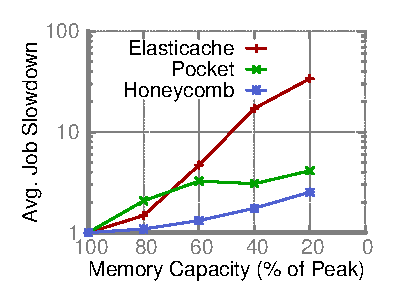
\includegraphics[width = 0.45\textwidth]{fig/jiffy/perfvcap}
    \label{fig:perfvcap}
  }
  \subfigure[Resource utilization] {
    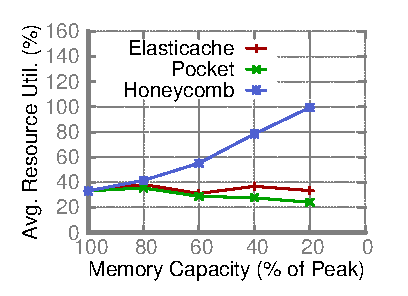
\includegraphics[width = 0.45\textwidth]{fig/jiffy/utilvcap}
    \label{fig:utilization}
  }
  \caption[Fine-grained task-level elasticity in \jiffy]{\textbf{Fine-grained task-level elasticity in \jiffy} enables (a) better job performance, and (b) higher resource utilization under constrained capacity. In (a), the slowdown is computed relative to the job completion time with $100\%$ capacity (for this data point, Elasticache performance was $30\%$ worse than Pocket, and Pocket performance was $5\%$ worse than \jiffy). See \S\ref{ssec:overallbenefits} for details.}
  \label{fig:elasticity}\vspace{-1.25em}
\end{figure}


\subsection{Benefits of \jiffy}
\label{ssec:overallbenefits}

\jiffy enables fine-grained resource allocation for serverless analytics. We demonstrate its impact on job performance and resource utilization across approximately 50,000 jobs from 100 randomly selected tenants over a 5-hour window in the Snowflake workload\footnote{We did not evaluate the full 14-day window with $>2000$ tenants due to intractable cost overheads.}~\cite{snowset}.

We compare \jiffy (using the MR programming model, \S\ref{ssec:jiffymodels}) with Elasticache~\cite{elasticache} and Pocket~\cite{pocket}. Elasticache provisions resources for \textit{all} jobs, and if capacity is insufficient, jobs must spill data to external stores like S3~\cite{s3}. Pocket, however, reserves and reclaims resources at a \textit{job} granularity, spilling data to SSD if DRAM capacity is insufficient. Pocket’s utilization can be lower than Elasticache, as it provisions separately for the peak demand of each job, which sacrifices overall utilization. To ensure a fair comparison, Pocket’s control and metadata services are colocated on the same server, similar to \jiffy’s unified control plane.

\paragraphb{Impact of fine-grained elasticity on job performance} We examine job performance under constrained intermediate storage capacity in the Snowflake workload. Figure~\ref{fig:perfvcap} shows the average job slowdown as capacity is reduced to a fraction of peak utilization. With Elasticache, performance drops sharply when data exceeds capacity, leading to a $34\times$ slowdown at 20\% capacity due to reliance on S3. Pocket experiences a $>4.1\times$ slowdown at 20\% capacity as it spills data to SSD. In contrast, \jiffy’s task-level elasticity and lease-based storage reclamation reduce data spilling, resulting in a much lower slowdown ($<2.5\times$ at 20\% capacity). This is because \jiffy multiplexes capacity more efficiently across jobs, minimizing reliance on slower storage tiers.

\paragraphb{Impact of fine-grained elasticity on resource utilization} Figure~\ref{fig:utilization} shows resource utilization under constrained capacity. While Elasticache and Pocket see reduced or stagnant utilization as capacity is constrained, \jiffy’s utilization \textit{improves}. Elasticache and Pocket allocate capacity at a job or coarser granularity, wasting unused resources regardless of total system capacity. In contrast, \jiffy’s fine-grained elasticity and lease-based reclamation allow it to multiplex capacity more effectively, reducing SSD spillover and improving performance as shown in Figure~\ref{fig:perfvcap}.


\begin{figure}
  \centering
  \subfigure[Latency] {
    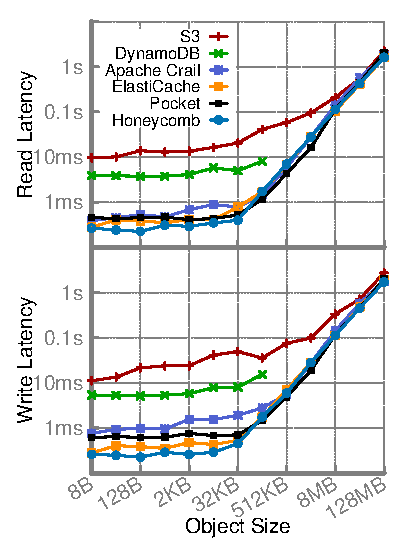
\includegraphics[width = 0.45\textwidth]{fig/jiffy/rw_latency}
    \label{fig:rwlatency}
  }%
  \subfigure[MBPS] {
    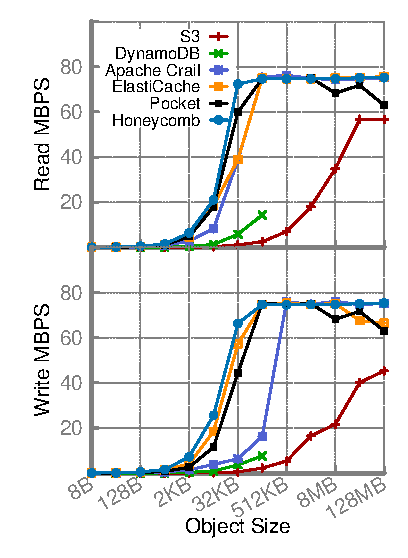
\includegraphics[width = 0.45\textwidth]{fig/jiffy/rw_mbps}
    \label{fig:rwmbps}
  }%
  \caption[\jiffy performance comparison with existing storage systems]{\small{\textbf{\jiffy performance comparison with existing storage systems (\S\ref{ssec:hrelated}).} Despite providing the additional benefits demonstrated in \S\ref{ssec:overallbenefits}, \jiffy performs as well as or outperforms state-of-the-art storage systems for serverless analytics.}}
  \label{fig:storage-perf}
\end{figure}

\subsection{Performance Benchmarks for Six Systems}
\label{ssec:hrelated}

We now compare \jiffy’s performance (using its KV-Store data structure) against five state-of-the-art systems commonly used for intermediate data storage in serverless analytics: S3, DynamoDB, Elasticache, Apache Crail, and Pocket. Since only a subset of these systems support request pipelining, we disable pipelining across all of them for consistency.

To measure latency and throughput, we profiled synchronous operations issued from an AWS Lambda instance using a single-threaded client. Figure~\ref{fig:storage-perf} shows that in-memory data stores like Elasticache, Pocket, and Apache Crail achieve low latency (sub-millisecond) and high throughput. In contrast, persistent data stores like S3 and DynamoDB exhibit significantly higher latencies and lower throughput; note that DynamoDB only supports objects up to $128$KB. \jiffy matches the performance of these in-memory data stores while also providing the additional benefits discussed in \S\ref{ssec:overallbenefits}.


\begin{figure*}[t]
  \centering
  \subfigure[Efficient lifetime management] {
    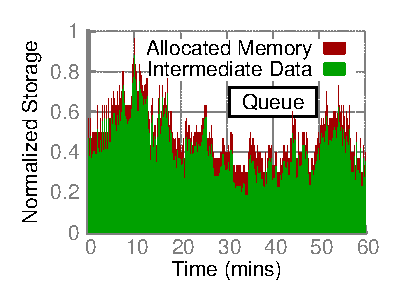
\includegraphics[width = 0.2\textwidth]{fig/jiffy/fifo_queue_scale_uniform}\hspace{-.5em}%
    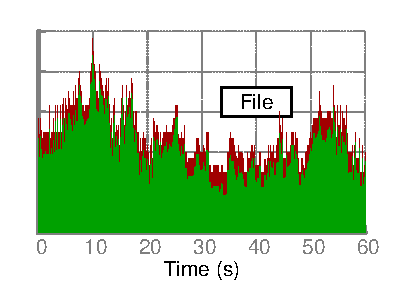
\includegraphics[width = 0.2\textwidth]{fig/jiffy/file_scale_uniform}\hspace{-.5em}%
    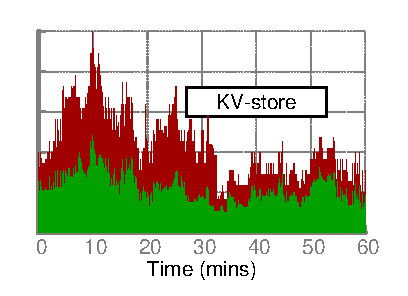
\includegraphics[width = 0.2\textwidth]{fig/jiffy/scale_zipf}
    \label{fig:fi-scale}
    \label{fig:ht-scale}
    \label{fig:fq-scale}
  }%
  \subfigure[Efficient data repartitioning] {
    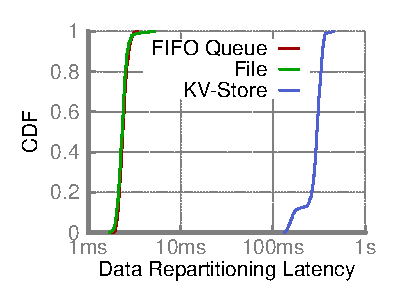
\includegraphics[width = 0.2\textwidth]{fig/jiffy/scale_latency_cdf}\hspace{-1.5em}%
    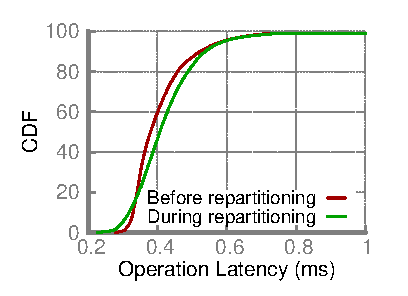
\includegraphics[width = 0.2\textwidth]{fig/jiffy/hash_table_scaling_get}
    \label{fig:op-latency-scaling}
    \label{fig:scale-latency}
  }
  \caption[\jiffy data lifetime-management and data repartitioning]{\textbf{\jiffy data lifetime-management and data repartitioning.} (a) \jiffy provides fine-grained elasticity through lease-based lifetime management for its built-in data structures: FIFO Queue (left), File (center), and KV-store (right). It efficiently reclaims resources from tasks once their leases expire. (b) \jiffy enables efficient data repartitioning as allocations scale up, with repartitioning for a single block completing within $2$-$500$ms (left). Additionally, the latency for 100KB \texttt{get} operations is minimally affected during KV-store repartitioning. Note: plots in (a) and (b) share a common y-axis; the x-axis for (c, left) is in log scale.}
\end{figure*}


\subsection{Understanding \jiffy Benefits}
\label{ssec:jiffybenefits}

Figure~\ref{fig:elasticity} demonstrates how \jiffy's fine-grained elasticity provides performance and resource utilization advantages over other state-of-the-art systems. This elasticity is achieved through hierarchical virtual addressing, flexible data lifetime management, and data repartitioning. In this section, we isolate and evaluate the impact of these mechanisms.

\paragraphb{Fine-grained elasticity via data lifetime management} Unlike traditional storage systems, \jiffy’s lease-based data lifetime management enables the reclamation of unused resources, reallocating them to jobs in need. Coupled with fine-grained resource allocations and efficient data repartitioning, this enables elasticity for serverless jobs. To evaluate this, we examine storage allocation across various \jiffy data structures (Figure~\ref{fig:fq-scale}) using the Snowflake workload from Figure~\ref{fig:ephemerals}.

FIFO queue and file data structures exhibit seamless elasticity as intermediate data is written to them, as they do not require repartitioning. The allocated capacity slightly exceeds the intermediate data size, accounting for block metadata (e.g., object metadata for FIFO queue items) and unused space in head/tail blocks. For the KV-store, inserted keys are sampled from a Zipf distribution since the Snowflake dataset lacks access patterns. Due to the skew, some \jiffy blocks receive most key-value pairs and frequently split when their capacity grows too high, leading to higher allocated capacity. However, \jiffy’s lease mechanism quickly reclaims resources after their utility ends, ensuring that overheads are temporary.

\paragraphb{Efficient elastic scaling via flexible data repartitioning} A key factor in \jiffy’s elasticity is its efficient data repartitioning. Figure~\ref{fig:scale-latency} shows the CDF of repartitioning latency per block across the three data structures under the Snowflake workload. The latency includes the time from detecting an overloaded/underloaded block to the completion of repartitioning. Storage servers take ${\sim}1$-$1.5$ms to connect to the controller, with two round trips ($100$-$200\mu$s in EC2) to trigger block allocation/reclamation and update partitioning metadata. Unlike FIFO Queue and File, KV-Store requires data repartitioning across blocks, but since only half the block capacity (${\sim}64$MB) is moved, \jiffy completes repartitioning in a few hundred milliseconds over $10$Gbps links, achieving block-level repartitioning with low latency ($2$-$500$ms).

Importantly, \jiffy does not block data structure operations during repartitioning. As shown in Figure~\ref{fig:op-latency-scaling}, the CDF of 100KB \texttt{get} operations in the KV-Store before and during scaling remains almost identical, indicating minimal impact on operation latency during scaling.


\begin{figure}[h]
  \centering
  \subfigure[Controller throughput vs. latency on a single CPU core.] { 
    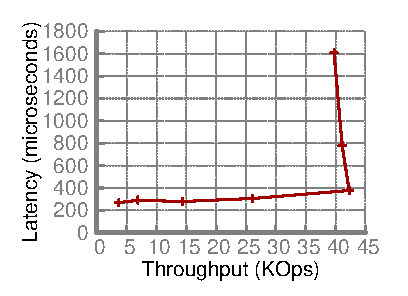
\includegraphics[width = 0.45\textwidth]{fig/jiffy/controller_tvl}
    \label{fig:controller-tvl}
  }
  \subfigure[Controller throughput scaling with multiple cores.] {
    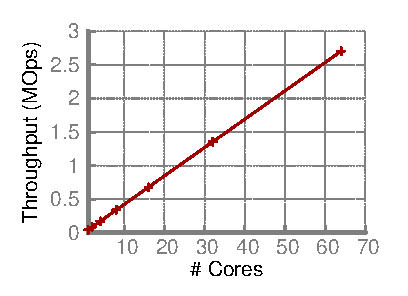
\includegraphics[width = 0.45\textwidth]{fig/jiffy/controller_scale}
    \label{fig:controller-scaling}
  }
  \caption[\jiffy controller performance]{{\textbf{\jiffy controller performance.} Details in Appendix~\ref{ssec:controller-scale}.}}
  \label{fig:controller-perf}
\end{figure}

\subsection{Controller Overheads}
\label{ssec:controller-scale}

\jiffy introduces several additional components at the controller compared to Pocket, including metadata management, lease management, and handling data repartitioning requests. As a result, its performance is expected to be lower than Pocket's metadata server. However, this is acceptable as long as \jiffy can manage the typical control plane request rates observed in real-world workloads, such as the peak of a few hundred requests per second—including lease renewals—seen in our evaluations and those in~\cite{pocket}.

Figure~\ref{fig:controller-tvl} shows the throughput-versus-latency curve for \jiffy controller operations on a single CPU core of an m4.16xlarge EC2 instance. The controller throughput saturates at around $42$ KOps with a latency of $370\mu$s. While this is lower than Pocket's throughput (~$90$ KOps per core), it is more than sufficient to handle the control plane load of real-world workloads. Additionally, throughput scales almost linearly with the number of cores, as each core processes requests independently for distinct subsets of virtual address hierarchies (Figure~\ref{fig:controller-scaling}). Finally, the control plane can scale across multiple servers by partitioning the address hierarchies.

\paragraphb{Storage overheads} The task-level metadata storage in Honeycomb has a minimal overhead of just 64 bytes of fixed metadata per task and 8 bytes per block. For \jiffy's default 128MB blocks, this results in an insignificant storage overhead ($<0.00005-0.0001\%$ of total storage).


\begin{figure*}[t]
  \centering
  \subfigure[Sensitivity analysis for block size] {
    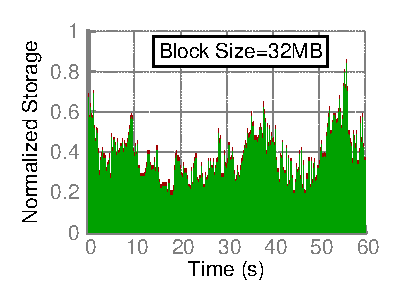
\includegraphics[width = 1.4in]{fig/jiffy/block_size_32}\hspace{-.5em}%
    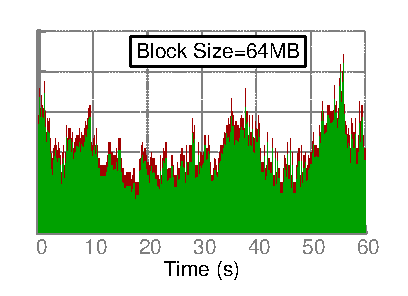
\includegraphics[width = 1.4in]{fig/jiffy/block_size_64}\hspace{-.5em}%
    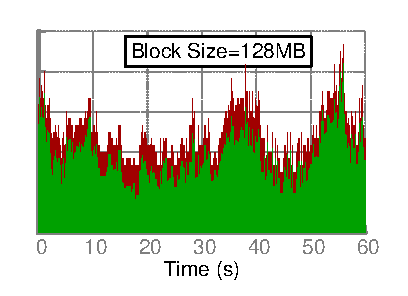
\includegraphics[width = 1.4in]{fig/jiffy/block_size_128}\hspace{-.5em}%
    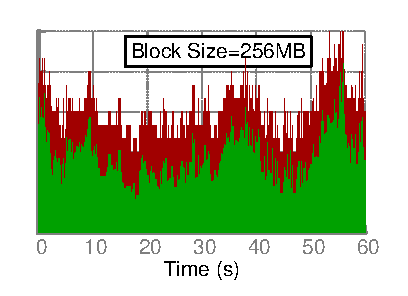
\includegraphics[width = 1.4in]{fig/jiffy/block_size_256}\hspace{-.5em}%
    %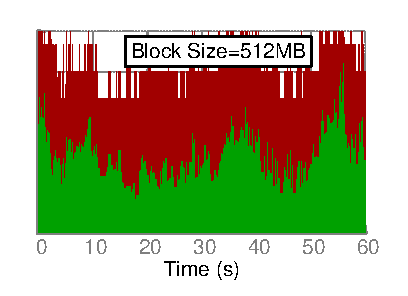
\includegraphics[width = 1.4in]{fig/jiffy/block_size_512}
    \label{fig:block-size}
  }
  \subfigure[Sensitivity analysis for lease duration] {
    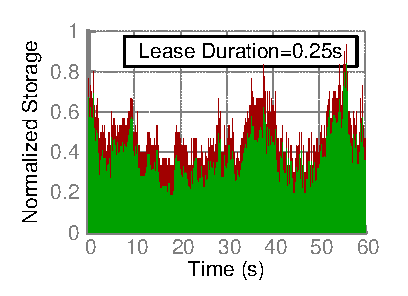
\includegraphics[width = 1.4in]{fig/jiffy/lease_duration_0_25}\hspace{-.5em}%
    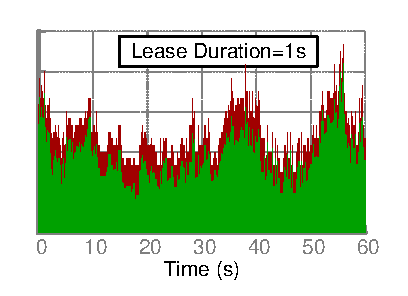
\includegraphics[width = 1.4in]{fig/jiffy/lease_duration_1}\hspace{-.5em}%
    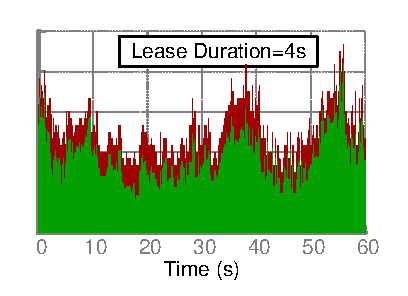
\includegraphics[width = 1.4in]{fig/jiffy/lease_duration_4}\hspace{-.5em}%
    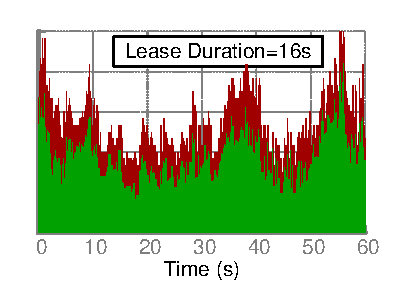
\includegraphics[width = 1.4in]{fig/jiffy/lease_duration_16}\hspace{-.5em}%
    %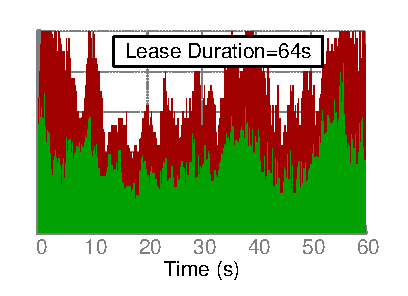
\includegraphics[width = 1.4in]{fig/jiffy/lease_duration_64}
    \label{fig:lease-duration}
  }
  \subfigure[Sensitivity analysis for (high) repartition threshold] {
    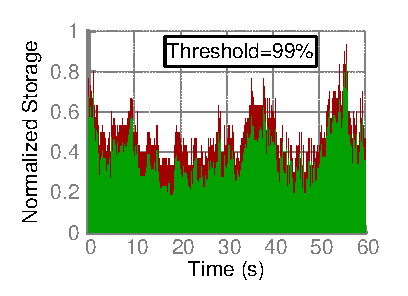
\includegraphics[width = 1.4in]{fig/jiffy/threshold_0_99}\hspace{-.5em}%
    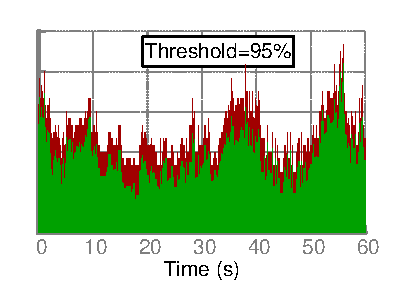
\includegraphics[width = 1.4in]{fig/jiffy/threshold_0_95}\hspace{-.5em}%
    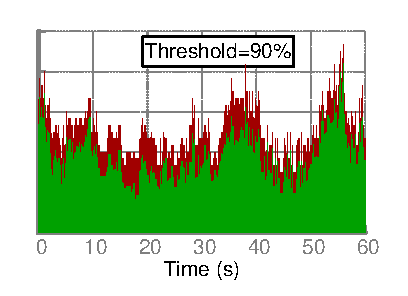
\includegraphics[width = 1.4in]{fig/jiffy/threshold_0_9}\hspace{-.5em}%
    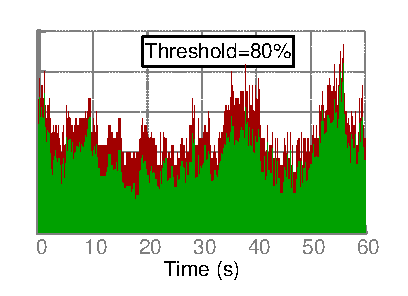
\includegraphics[width = 1.4in]{fig/jiffy/threshold_0_8}\hspace{-.5em}%
    %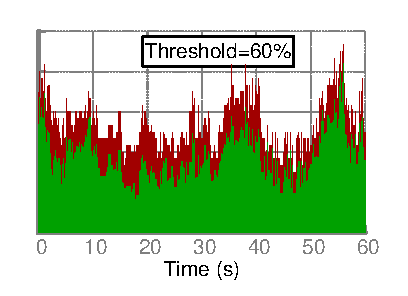
\includegraphics[width = 1.4in]{fig/jiffy/threshold_0_6}
    \label{fig:threshold}
  }
  \caption[\jiffy sensitivity analysis]{\textbf{\jiffy sensitivity analysis} for (a) block size (b) lease duration and (c) repartition threshold for the file data structure. Green area corresponds to used capacity, while red area corresponds to allocated capacity under \jiffy. See Appendix~\ref{ssec:jiffysensitivity} for details.}
\end{figure*}


\subsection{Sensitivity Analysis}
\label{ssec:jiffysensitivity}

We now perform sensitivity analysis for various system parameters in \jiffy, including block size (\S\ref{ssec:hva}), lease duration (\S\ref{ssec:mlm}) and thresholds for data repartitioning (\S\ref{ssec:fdr}). We use files as our underlying data structure, and use the Snowflake workload from Figure~\ref{fig:ephemerals}. These results can be contrasted directly with Figure~\ref{fig:fi-scale}~(center), which corresponds to our default system parameters ($128$MB blocks, $1$s lease duration and $95\%$ of block occupancy as repartition threshold). For each parameter that we vary, the other to remain fixed at their default values.

\paragraphb{Block size (Figure~\ref{fig:block-size})} As discussed in \S\ref{ssec:hva}, the block size in \jiffy exposes a tradeoff between the amount of metadata that needs to be stored at the control plane, and resource utilization. This is confirmed in Figure~\ref{fig:block-size}, where increasing the block size from $32$MB to $256$MB increases the disparity between allocated and used capacity, and therefore decreases the resource utilization. The default block size in \jiffy is set to $128$MB for two main reasons: (1) it allows high enough utilization with low enough metadata overhead (a few megabytes for even thousands of gigabytes of application data), and (2) it is the default block size used in existing data analytics platforms; as such, $128$MB blocks ensure seamless compatibility with such frameworks.

\paragraphb{Lease duration (Figure~\ref{fig:lease-duration})} As shown in Figure~\ref{fig:lease-duration}, lease duration in \jiffy controls resource utilization over time. As we increase lease durations from $0.25$ seconds to $16$ seconds, resource utilization increases since \jiffy does not reclaim (potentially unused) resource resources from jobs until their leases expire. At the same time, if we keep lease duration too low, applications would renew leases too often, resulting in higher traffic to the \jiffy controller. We find a lease duration of $1$s to be a sweet spot, ensuring high enough resource utilization, while ensuring the number of lease requests for even thousands of concurrent applications is only a few thousand requests per second --- well within \jiffy controller's limits on a single CPU core.

\paragraphb{Repartition threshold (Figure~\ref{fig:threshold})} Finally, Figure~\ref{fig:threshold} shows the impact of (high) repartition threshold on resource utilization. As expected, lowering the repartition threshold leads to poor utilization, since it triggers pre-mature allocation of new blocks to most files in our evaluated workload. However, since the size of the block ($128$MB) is much smaller than the amount of data written to each file in the workload (often several gigabytes), this overhead is relatively small when compared to effect of other parameters. However, a larger value of high repartitioning threshold results in more frequent block allocation requests to the controller; we find that our default value of $95\%$ provides a reasonable compromise between resource utilization and number of control plane requests.


\section{Related Work}
Pocket~\cite{pocket} demonstrates how existing designs for in-memory key-value stores~\cite{redis, farm, memcached, memc3, mica, ramcloud, anna, succinct, blowfish}, distributed~\cite{dsm1, dsm2, dsm3, treadmarks}, and disaggregated memory systems~\cite{infiniswap,remoteregions,legoos,mind}, as well as storage systems with flexible interfaces~\cite{udf1, udf2, udf3, storedprocedure1, storedprocedure2, storedprocedure3, boxwood, sinfonia}, can be adapted to achieve three primary goals for intermediate data storage in serverless analytics: low-latency/high-throughput, resource sharing, and elasticity.

Other recent systems have also explored fine-grained resource sharing. Pisces~\cite{pisces} provides per-tenant performance isolation in multi-tenant cloud storage systems but does not share storage capacity across tenants. Memshare~\cite{memshare} facilitates memory sharing across tenants in a KV cache setting, though it evicts KV pairs with lower contribution to hit-rate under high contention.


\section{Summary}
\label{sec:jiffysummary}
In this chapter, we have presented \jiffy, a memory management service designed for disaggregated memory, allocating memory in small fixed-size blocks. These blocks store intermediate data for individual tasks within a job. Inspired by virtual memory systems in operating systems, \jiffy scales memory resources elastically without prior knowledge of data sizes, adapting to job demands in real-time. This approach allows \jiffy to efficiently share fast memory across jobs, reducing reliance on slower secondary storage such as S3.








